\documentclass[10pt,a4paper]{article}
\usepackage[margin=2.2cm]{geometry}
\usepackage{fontspec}
\usepackage{kotex}
\setmainfont{Apple SD Gothic Neo}
\setsansfont{Apple SD Gothic Neo}
\usepackage{amsmath,amssymb}
\usepackage{graphicx}
\usepackage{booktabs}
\usepackage{caption}
\usepackage[dvipsnames]{xcolor}
\usepackage[colorlinks=true,linkcolor=MidnightBlue,citecolor=MidnightBlue,
            urlcolor=MidnightBlue]{hyperref}
\usepackage{titlesec}
\titleformat{\section}{\large\bfseries}{\thesection}{0.6em}{}
\titleformat{\subsection}{\normalsize\bfseries}{\thesubsection}{0.5em}{}
\captionsetup{font=small,labelfont=bf}
\setlength{\parskip}{0.35em}
\setlength{\parindent}{0pt}

\usepackage{mdframed}
\newmdenv[linewidth=0.4pt,linecolor=gray!60,backgroundcolor=gray!5,
          innertopmargin=6pt,innerbottommargin=6pt,skipabove=8pt,skipbelow=8pt]{claimbox}
\newcommand{\claim}[2]{\begin{claimbox}\textbf{주장.} #1\par\smallskip
  \textcolor{gray!70}{\textbf{반증 조건.} #2}\end{claimbox}}

\title{\bfseries 면허가 배선이 됐다\\[2pt]
\large absolute() --- 승격을 카드 문장에서 창구 기능으로}
\author{월드모델 실험실 · 노트 $809$}
\date{2026-08-07}
\begin{document}\maketitle

\section{한 줄}

논문 $166$ 이 남긴 빚 --- \emph{``서빙 층이 아직 이것을 물지 않는다. 그때까지
승격은 카드 위의 문장이다''} --- 을 갚았다. \texttt{warm()} 이 T$=2023$ 적합을
한 번 더 해 $8$개 도메인의 \textbf{안 옮김 $+$ 학습 예보 분포 $+$ 학습 라벨}을
캐시에 굽고(지문 v$3$ · \texttt{lab/calib.py} 편입), 창구
\texttt{absolute(domain, query)} 와 MCP \texttt{abs\_corrected} 가 생겼다.

\textbf{받아들임 격자 $6/6$}: ① 캐시 적중 $0.02$초 · 보정 도메인 정확히 $8$개
② 게임 스팟 --- \texttt{absolute} $9.876 =$ 직접 재계산 $9.876$ · 자 문구 포함
③ 도서 거부 $+$ 도메인 구간 대안 ④ \texttt{capability.check} 통과($12/12$ 유지)
⑤ \texttt{calib.py} 수정 $\to$ 캐시 거부 ⑥ 데우기 $155{\sim}169$초(f$23$ 추가분
$\approx 90$초).

\begin{figure}[t]\centering
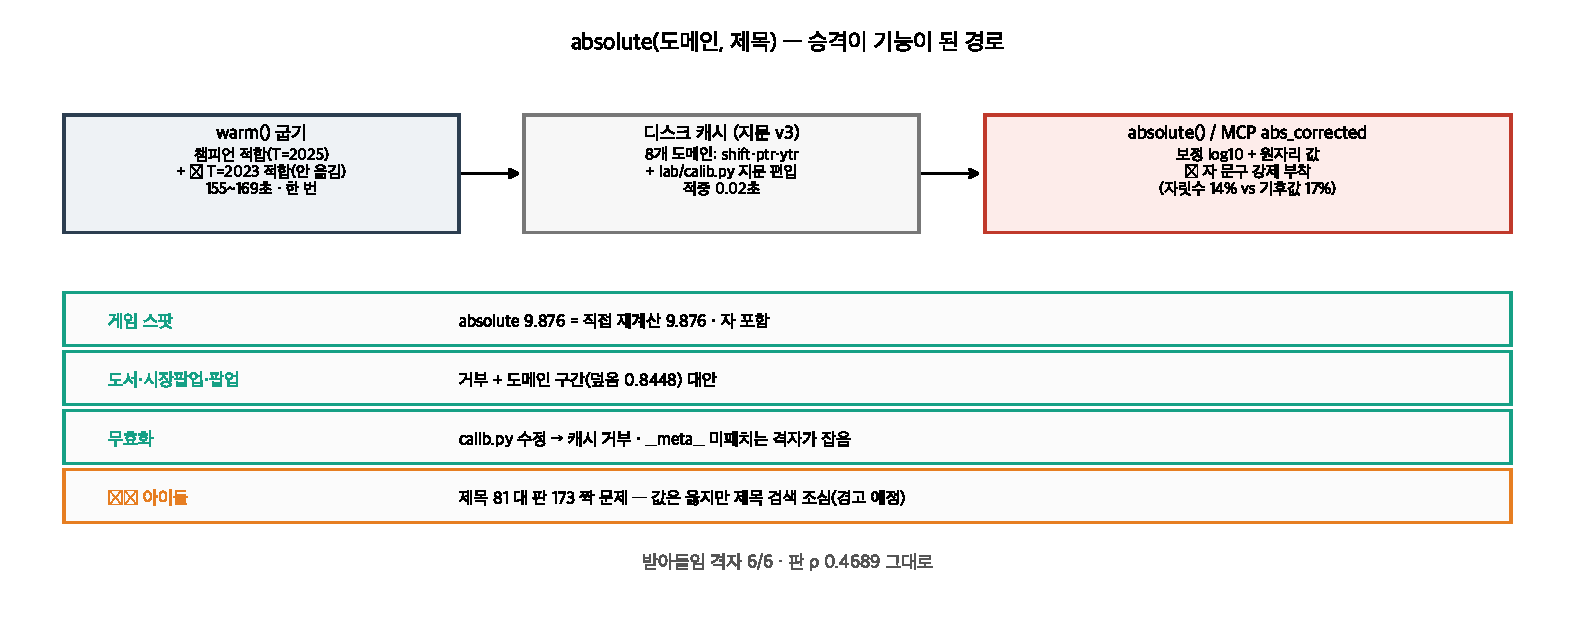
\includegraphics[width=0.95\textwidth]{figs/wire.pdf}
\caption{경로와 격자 --- 마지막 줄이 남긴 빚(아이돌 제목 짝)이다.}
\end{figure}

\section{금지의 시행이 코드가 됐다}

\claim{\textbf{자 문구는 옵션이 아니라 반환의 일부다} --- \texttt{ABS\_RULER}
(``자릿수를 $14\%$ 확률로 틀립니다 · 평균만 말하면 $17\%$'')가 모든 성공 반환에
붙고, 보정 없는 세 도메인은 \textbf{창구가 거부하며 도메인 구간(덮음 $0.8448$)을
대안으로 낸다.} 능력 카드의 금지 꼴(``맨 절대값'')을 사람 기억이 아니라 서빙이
시행한다 --- 감사표 $2$행이 이 코드를 지킨다.}
{빠져나갈 길은 남아 있다 --- 부르는 쪽(에이전트·사람)이 반환에서 숫자만 떼어
말하면 금지 꼴이다. \texttt{capability.check} 가 창구 출력을 훑지만 대화 전체를
훑지는 못한다.}

\section{도중에 잡은 것 둘과 남긴 것 하나}

\claim{격자가 일을 했다: (a) \texttt{\_\_meta\_\_} 패치가 들여쓰기 불일치로 안
먹어 \textbf{blob 만 구워지고 메타가 옛것}이었다 --- 격자 ①(보정 도메인 $0$개)이
잡았고 \texttt{assert} 로 고쳤다. (b) \textbf{``사람 수 자리로''가 오표기였다}
--- 라벨의 뜻은 도메인마다 다르다(팝업$=$방문객 · 게임$=$리뷰 창 · 만화$=$인기
지표). ``원자리 값(라벨 정의는 도메인마다 다름)''으로 정정했다 --- \textbf{같은
숫자도 이름이 틀리면 거짓이 된다.}}
{\textbf{남긴 빚}: 아이돌 제목 배열($81$)과 판 행($173$)의 어긋남(노트 $789
\cdot 805$)이 여기도 적용된다 --- \textbf{값 계산은 옳지만 제목-행 짝이 틀릴 수
있다.} T$1$ 의 배선 수리 전까지 아이돌 \texttt{absolute} 에 경고를 박는 것이
다음 사이클의 싼 일이다.}

\section{T$6$ 이 닫혔다}

$791$(진단) $\to$ $792$(전이적 상쇄) $\to$ $800$(예측 가능성) $\to$ $801$(보정)
$\to$ $802$(확인·승격) $\to$ $808$(승부 가르기 --- 모름) $\to$ $809$(배선).
\textbf{T$6$ 에 잴 것이 남지 않았다.} 판 $\rho$ 는 아홉 걸음 내내 $0.4689$
그대로였고, 이 트랙이 세션에 남긴 것은 순위가 아니라 \textbf{말할 수 있는 것의
정확한 지도}다.

\end{document}
